%%%%%%%%%%%%%%%%%%%%%%%%%%%%%%%%%%%%%%%%%%%%%%%%%%%%%%%%%%%%%%%%%%%%%%%%%%%%%%%%
%2345678901234567890123456789012345678901234567890123456789012345678901234567890
%        1         2         3         4         5         6         7         8

\documentclass[journal]{IEEEtranTIE}

% See the \addtolength command later in the file to balance the column lengths
% on the last page of the document

% The following packages can be found on http:\\www.ctan.org
%\usepackage{graphicx}
\usepackage{graphics} % for pdf, bitmapped graphics files
\usepackage{epsfig} % for postscript graphics files
\usepackage{subcaption}
\usepackage[noadjust]{cite}
%\usepackage{mathptmx} % assumes new font selection scheme installed
%\usepackage{times} % assumes new font selection scheme installed
\usepackage{algorithm,algpseudocode}
\usepackage{gensymb} % enable the use of degree symbol
\usepackage{amsmath,amssymb,amsfonts,amsthm} % assumes amsmath package installed
%\usepackage{booktabs}

% format for theorems etc.
\newtheorem{thm}{\bfseries Theorem}
\newtheorem{lem}{\bfseries Lemma}
\newtheorem{cor}{\bfseries Corollary}
\newtheorem{prop}{\bfseries Proposition}
\theoremstyle{remark}
\newtheorem{rem}{\bfseries Remark}
%\newtheorem*{proof*}{\bfseries Proof}

% format for argmin, argmax
\newcommand{\argmax}{\operatornamewithlimits{argmax}}

% format for cross-reference
\usepackage[capitalize]{cleveref}
\crefname{equation}{eq.}{eq.}
\Crefname{equation}{Eq.}{Eq.}
\crefname{thm}{theorem}{theorems}
\Crefname{thm}{Theorem}{Theorems}
\crefname{lem}{lemma}{lemmas}
\Crefname{lem}{Lemma}{Lemmas}
\crefname{cor}{corollary}{corollaries}
\Crefname{cor}{Corollary}{Corollaries}
\crefname{prop}{proposition}{propositions}
\Crefname{prop}{Proposition}{Propositions}
\crefname{rem}{remark}{remarks}
\Crefname{rem}{Remark}{Remarks}

%=====todonotes===== %
\usepackage{todonotes}
\usepackage{soul}
\definecolor{smoothgreen}{rgb}{0.7,1,0.7}
\sethlcolor{smoothgreen}

\newcommand{\todopara}[1]{\vspace{0px} %
	\todo[inline, color=black!10]{\textbf{[Paragraph:]} {#1}} %
}
\newcommand{\todonote}[1]{\vspace{0px} %
	\todo[inline, color=green!30]{\textbf{[Note:]} {#1}} %
}
\newcommand{\todoQ}[1]{\vspace{0px} %
	\todo[inline, color=orange!50]{\textbf{[Note:]} {#1}} %
}
\newcommand{\todohere}[1]{\hl{(\textbf{TODO:} #1)}}

\newcommand{\hidetodos}{
	\renewcommand{\todopara}[1]{}
	\renewcommand{\todonote}[1]{}
	\renewcommand{\todoQ}[1]{}
	\renewcommand{\todohere}[1]{}
	}

%---------- Macros for this paper
% random variables
\newcommand{\X}{X}
\newcommand{\Z}{Z}
\newcommand{\xg}{x^g}

\title{\LARGE \bf
	Supplementary Material}

\author{}

%\author{Chang Liu$^{1}$, Shengbo Eben Li$^{2}$ and J. Karl Hedrick$^{1}$% <-this % stops a space
%\thanks{*The first two authors, C. Liu and S. Li, have equally contributed to this research. All correspondence should be addressed to S. Li. The work is supported by the ONR MURI project and the NSF China with grant 51575293 and 51622504.
%	}% <-this % stops a space
%%\thanks{*This work is supported by the Embedded Humans: Provably Correct Decision Making for Networks of Humans and Unmanned Systems project, a MURI project funded by the Office of Naval Research and by the China National Science Foundation.}
%\thanks{$^{1}$Chang Liu and J. Hedrick are with the Department of Mechanical Engineering, University of California, Berkeley, Berkeley, CA 94709, USA. Email: {\tt\small changliu@berkeley.edu, khedrick@me.berkeley.edu}}%
%\thanks{$^{2}$S Li is now with the Department of Automotive Engineering, Tsinghua University, Beijing, 100084, China. He has worked at the Department of Mechanical Engineering, University of California, Berkeley. Email: {\tt\small lisb04@gmail.com}}%
%%\thanks{$^{3}$J. Karl Hedrick is with the Vehicle Dynamics \& Control Lab, Department of Mechanical Engineering, University of California, Berkeley, Berkeley, CA 94709, USA. Email: {\tt\small khedrick@me.berkeley.edu}}%
%}

\begin{document}

%\hidetodos % hide all todos 

\maketitle
\thispagestyle{empty}
\pagestyle{empty}

%\setlength{\belowcaptionskip}{-10pt} % set the spacing between figure and text

%%%%%%%%%%%%%%%%%%%%%%%%%%%%%%%%%%%%%%%%%%%%%%%%%%%%%%%%%%%%%%%%%%%%%%%%%%%%%%%%

\section{Simulation Verification for Target Localization}
Simulation has been conducted to evaluate the effectiveness of LIFO-DBF for target localization using a team of six UGVs.
%In all scenarios, each UGV is equipped with a binary sensor. 
The networked UGVs take a ring communication topology that each UGV can communicate with two fixed neighbors.
%The probabilistic sensor model
% \cref{eqn:bin_sensor1,eqn:bin_sensor0}, 
%takes the form defined in \Cref{eqn:gauss_sensor}.
%\small\begin{align}\label{eqn:gauss_sensor}
%\small\begin{subequations}\label{eqn:gauss_sensor}
%	\begin{align}
%		P(z^i_k=1|x_k^g;x_k^i)&=e^{-\frac{1}{2}(x_k^g-x_k^i)^T{\Sigma}^{-1}(x_k^g-x_k^i)}\\
%%		\exp\left\lbrace -\frac{1}{2}(x-x^R)^T{\Sigma}^{-1}(x-x^R)\right\rbrace \\
%		P(z^i_k=0|x_k^g;x_k^i)&=1-P(z^i_k=1|x_k^g;x_k^i),
%	\end{align}
%\end{subequations}\normalsize
%which reflects the fact that target detection becomes more probable as the UGV approaches the target position.
%\end{align}\normalsize
%where $x^s$ denotes the UGV position where current measurement is obtained. 
%Figure 4 shows the 1-D illustration of Gaussian binary sensor model.
%where $x^R$ denotes the UGV position, which is included in UGV state $y^R$.
DBF is implemented using the histogram filter method, by which the continuous space is finely discretized into finitely many regions and the individual PDF is approximated by the cumulative probability of each region \cite{thrun2005probabilistic}. 
%Other approaches, such as particle filters \cite{}, can also be used.
Two types of scenarios are used: in the first scenario, both UGVs and the target are static;
%, which acts as a proof of concept of LIFO-DBF for static target.
the second scenario subsequently deals with moving UGVs for localizing a moving target. 
In each scenario, we also test two different kinds of UGV team: the first UGV team, called the homogeneous team, is equipped with bearing-only sensors; in the second team, called the heterogeneous team, three UGVs are equipped with bearing-only sensor and the other three equipped with range-only sensors.
The bearing-only sensors are assumed to have large enough sensing range to cover the simulation field and the measurement noise is a zero-mean Gaussian white noise with standard deviation being $0.5$.
The range-only sensors are assumed to have $360\degree$ field of view and the measurement noise is a zero-mean Gaussian white noise with standard deviation being $5$.
%When the target is outside of the sensor's sensing range, an empty measurement is obtained, which is also used for updating the individual PDF.

In both scenarios, LIFO-DBF is compared with two commonly adopted approaches in multi-agent filtering: the consensus-based distributed filtering (CbDF) method \cite{olfati2006belief} and the centralized filtering (CF) method \cite{veeravalli2012distributed}.
The CbDF requires UGVs to continually exchange their individual PDFs with direct neighbors, computing the average of its own and the received PDFs. 
Multiple rounds of communication and averaging are conducted during the ``Sending Step'' and ``Receiving Step'' in Algorithm $1$ at each step to ensure the convergence of UGV's individual PDFs.
The CF assumes a central unit that can constantly receive and fuse all UGVs' latest measurements into a single PDF.
Ten test trials with randomly generated initial UGV and target positions are run and each trial is terminated after 50 time steps.
The average error between the estimated (using the MAP estimator) and true target position and the average entropy of individual PDFs of all 10 trials using these three approaches are compared.


\subsection{Static UGVs, Static Target}



%In this test, all UGVs are equipped with bearing-only sensors.\label{subsec:sim1}
The individual PDF of each UGV is initialized as a uniform distribution over a bounded space. 
At each time step, each UGV executes the LIFO-DBF for static target (Section III-B) to update their estimation of target position.
The evolution of the $1^\text{st}$ robot's individual PDF is shown in \Cref{fig:sta_sen_sta_tar_sing1,fig:sta_sen_sta_tar_sing2,fig:sta_sen_sta_tar_sing3,fig:sta_sen_sta_tar_sing4}. 
Since the robot is equipped with a noisy bearing-only sensor, the measurement at step $1$ results in a wide distribution with the peak centered along the noise-corrupted measured direction from the sensor to the target, as \Cref{fig:sta_sen_sta_tar_sing1} illustrates.
%six static UGVs, as represented by green stars and red square in , are placed in the field.
%The target is also assumed to be static, with $A$ being an identity matrix and $B_k$ being a zero matrix in \cref{eqn:tar_motion_model}.
% shows a test trial when both the UGVs and the target are static. %of the positions of six static UGVs are shown as stars and square.
%Due to space constraint, only the individual PDF of the first UGV is shown.
%The individual PDF of the first UGV at different time steps are shown in \cref{fig:sta_sen_sta_tar_sing1,fig:sta_sen_sta_tar_sing2,fig:sta_sen_sta_tar_sing3,fig:sta_sen_sta_tar_sing4}.
%Each UGV constantly receives binary measurements of the target.
%The LIFO-DBF for static target is implemented on each UGV for target localization.
%The networked UGVs use a ring communication topology that each UGV can communicate with two fixed neighbors.
%\cref{fig:sta_sen_sta_tar} shows the estimation results of the static target. 
%After the initial measurement, each UGV forms a circular individual PDF, centered at its own position.
%\cref{fig:sta_sen_sta_tar_sing1} shows the individual PDF after initial measurement for $1^\text{st}$ UGV.
%The circular PDF happens because the Gaussian sensor model (\Cref{eqn:gauss_sensor}) only depends on the distance between UGV and target.
As more measurements are fused, the individual PDF asymptotically concentrates to the true location of the target, which accords with the consistency of LIFO-DBF.
%In fact, with the Guassian sensor model (\Cref{eqn:gauss_sensor}), all positions with equal distance to a UGV belong to the same equi-parameter set of the UGV.
%Considering the system of six UGVs located separately, the equi-parameter set that contains the actual target position only contains one element.
%\cref{fig:entropy} (a) shows the decrease of the entropy of each UGV's individual PDF, indicating the reduction of the uncertainty in PDF estimation.

The \Cref{fig:sta_sen_sta_tar_pos_err,fig:sta_sen_sta_tar_entropy} shows the comparison of LIFO-DBF with CbDF and CF.
Unsurprisingly, the CF achieves the best performance in terms of both small position estimation error and fast reduction of entropy. 
This happens because the central unit has access to the latest measurements of all UGVs, thus being able to make the most use of all available information.
It is worth noting that, LIFO-DBF achieves similar asymptotic performance as the CF, both in position estimation error and entropy reduction; this is achieved even though each UGV only communicates with its two neighboring UGVs, which requires less communication burden than the CF.
The CbDF has the worst performance among these three filtering approaches. 
It results in slow reduction of entropy and the position error remains large.
This happens because Bayes filtering (Eq. $(3)$ and $(5)$) is a nonlinear process.
Using the linear average consensus law to fuse individual PDFs thus deviates from the actual Bayesian filtering and therefore cannot fully exploit the information of new measurements to reduce the uncertainty of estimation.

The \Cref{fig:htr_sta_sen_sta_tar} shows the simulation results of the heterogeneous team.
The individual PDF of the UGV with a noisy range-only sensor is presented in \Cref{fig:htr_sta_sen_sta_tar_sing1,fig:htr_sta_sen_sta_tar_sing2,fig:htr_sta_sen_sta_tar_sing3,fig:htr_sta_sen_sta_tar_sing4}.
At step $1$, the target is detected and the individual PDF is updated such that the peak of the  distribution centers at the positions whose distance to the sensor equals the noise-corrupted measured value. 
Similar to the case of using the homogeneous team, the individual PDF asymptotically concentrates to the true target position.
Due to the use of various sensors, the estimation accuracy increases faster than the homogeneous team case, as shown in \Cref{fig:htr_sta_sen_sta_tar_pos_err,fig:htr_sta_sen_sta_tar_entropy}.
It can also be noticed that, LIFO-DBF achieves similar performance as CF, while the performance of CbDF is the worst.

%
\subsection{Moving UGVs, Moving Target}

In this scenario, each UGV follows a pre-defined circular trajectory. 
The target motion is modeled as a single-integrator with unit velocity on both directions.
Each UGV executes the LIFO-DBF for moving target (Section III-C) for estimation.
\Cref{fig:mov_sen_mov_tar_sing1,fig:mov_sen_mov_tar_sing2,fig:mov_sen_mov_tar_sing3,fig:mov_sen_mov_tar_sing4} and \Cref{fig:htr_mov_sen_mov_tar_sing1,fig:htr_mov_sen_mov_tar_sing2,fig:htr_mov_sen_mov_tar_sing3,fig:htr_mov_sen_mov_tar_sing4} illustrate the evolution of individual PDF for homogeneous and heterogeneous teams, respectively.
They all present similar asymptotic behavior of individual PDFs as in aforementioned simulations.
%Note that \Cref{fig:htr_mov_sen_mov_tar_sing1} shows the individual PDF at step $1$ when the target is out of the sensing domain of the $5^\text{th}$ UGV's range-only sensor.
%It can be noticed that the individual PDF concentrates to the true target location when the target constantly moves.

\cref{fig:mov_sen_mov_tar_pos_err,fig:mov_sen_mov_tar_entropy} and \cref{fig:htr_mov_sen_mov_tar_pos_err,fig:htr_mov_sen_mov_tar_entropy} compare LIFO-DBF with CbDF and CF.
%Similar to results in \cref{subsec:sim1}, CF achieves best performance with smallest position estimation error and fastest entropy reduction; LIFO-DBF shows similar asymptotic performance as the CF; and
%CbDF has the slowest entropy reduction among all three filtering approaches.
It is worth noting that, for the heterogeneous team, CbDF achieves comparable position estimation error performance as the CF and LIFO-DBF.
%This is not an unexpected result: due to the consensus procedure, CbDF is able to fuse the latest individual PDFs of each UGV via the averaging process. 
%This is especially useful when the environment is dynamically changing.
%In contrast, LIFO-DBF for each UGV only uses delayed information from neighboring UGVs, thus gaining less knowledge about the target's current position.
However, CbDF requires multiple rounds of exchanging individual PDFs, which incurs much higher communication burden than LIFO-DBF at each time step.
Considering the small difference in position estimation error and significantly faster entropy reduction, LIFO-DBF is still preferable over CbDF for moving target scenario.

\newpage

\begin{figure}[p]%[thpb]
	\centering
	\begin{subfigure}{0.23\textwidth}%[b]
		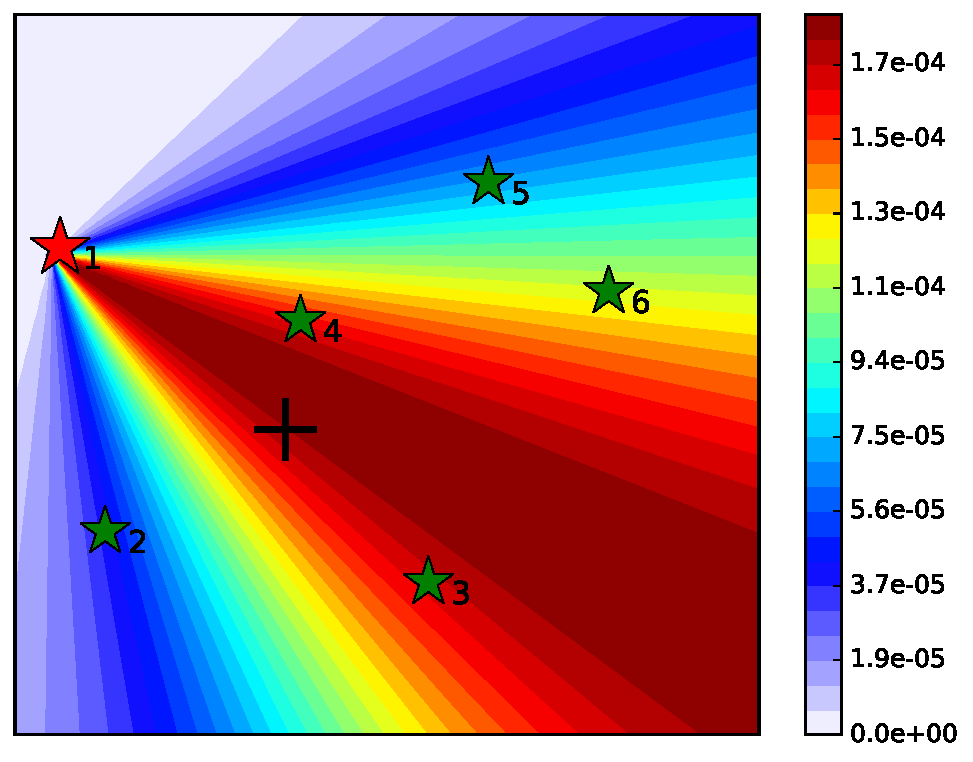
\includegraphics[width=\textwidth]{figures/brg_sta_sen_sta_tar_rbt1_step1}
		\caption{Step 1}\label{fig:sta_sen_sta_tar_sing1}
	\end{subfigure}
	\begin{subfigure}{0.23\textwidth}%[b]
		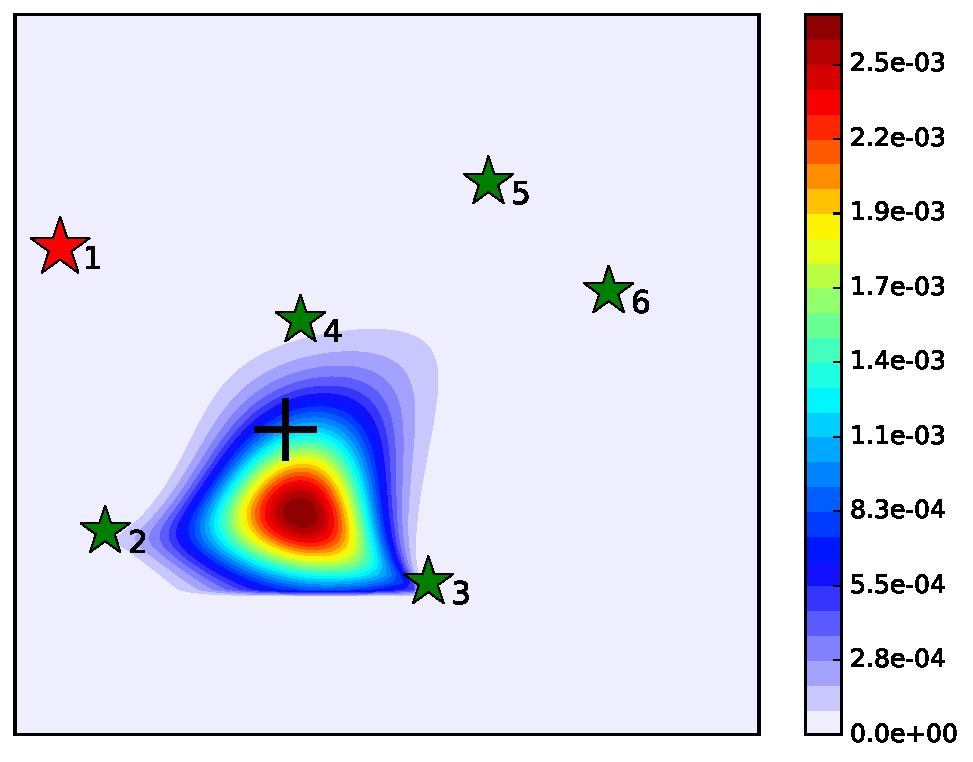
\includegraphics[width=\textwidth]{figures/brg_sta_sen_sta_tar_rbt1_step3}
		\caption{Step 3}\label{fig:sta_sen_sta_tar_sing2}
	\end{subfigure}
	\begin{subfigure}{0.23\textwidth}%[b]
		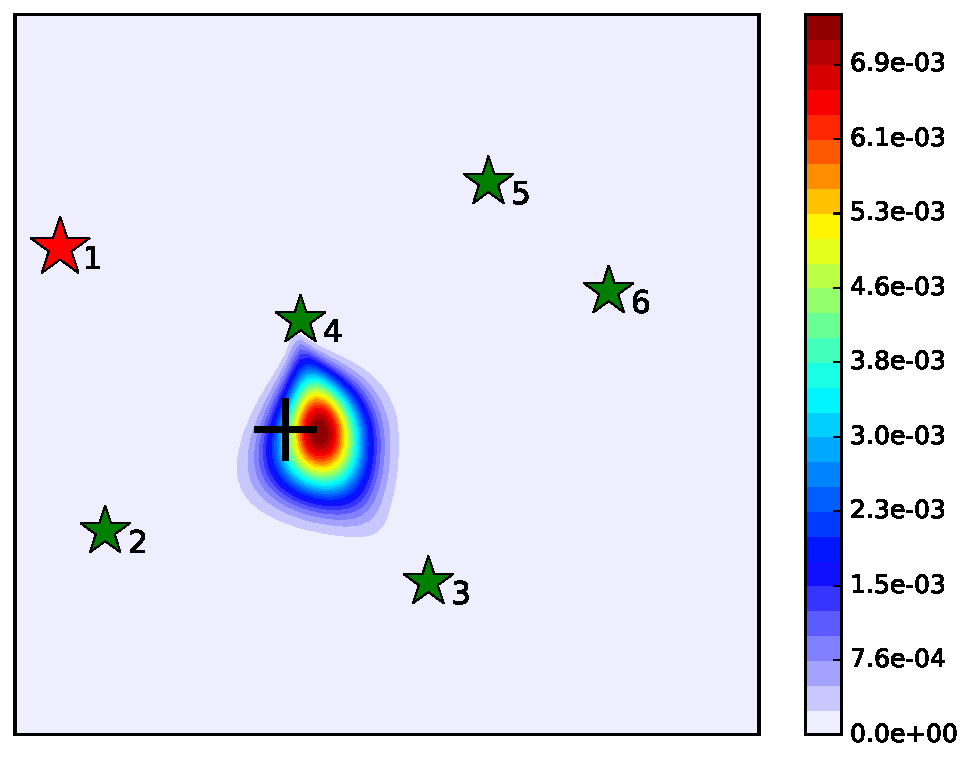
\includegraphics[width=\textwidth]{figures/brg_sta_sen_sta_tar_rbt1_step5}
		\caption{Step 5}\label{fig:sta_sen_sta_tar_sing3}
	\end{subfigure}
	\begin{subfigure}{0.23\textwidth}%[b]
		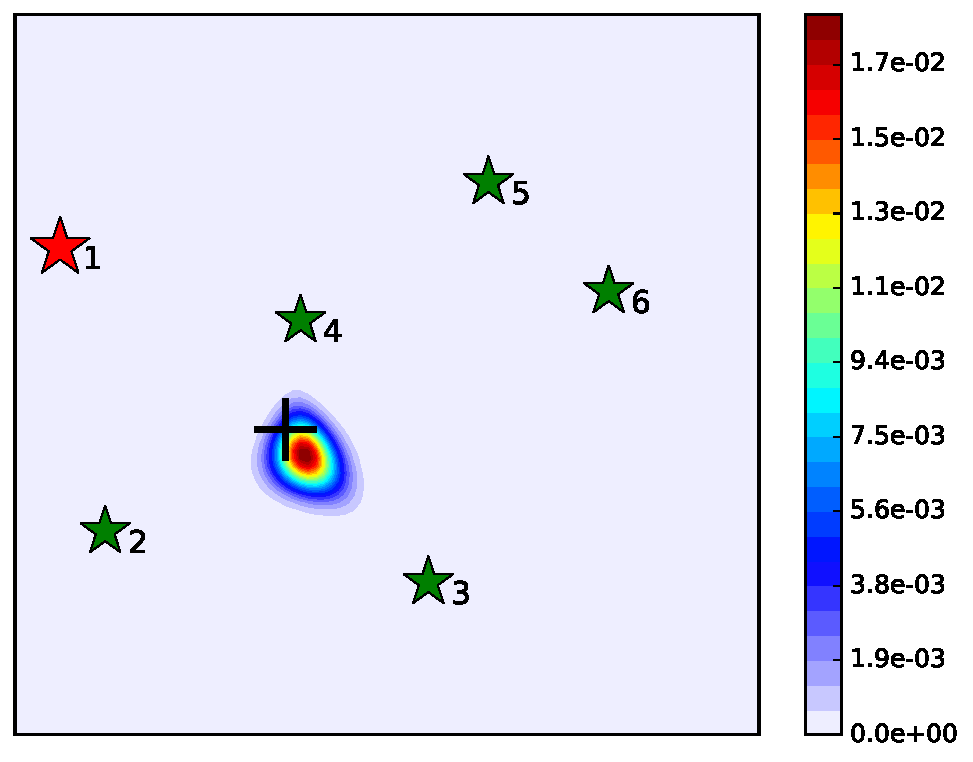
\includegraphics[width=\textwidth]{figures/brg_sta_sen_sta_tar_rbt1_step10}
		\caption{Step 10}\label{fig:sta_sen_sta_tar_sing4}
	\end{subfigure}
	\begin{subfigure}{0.23\textwidth}%[b]
		%		\includegraphics[width=\textwidth]{figures/test}
		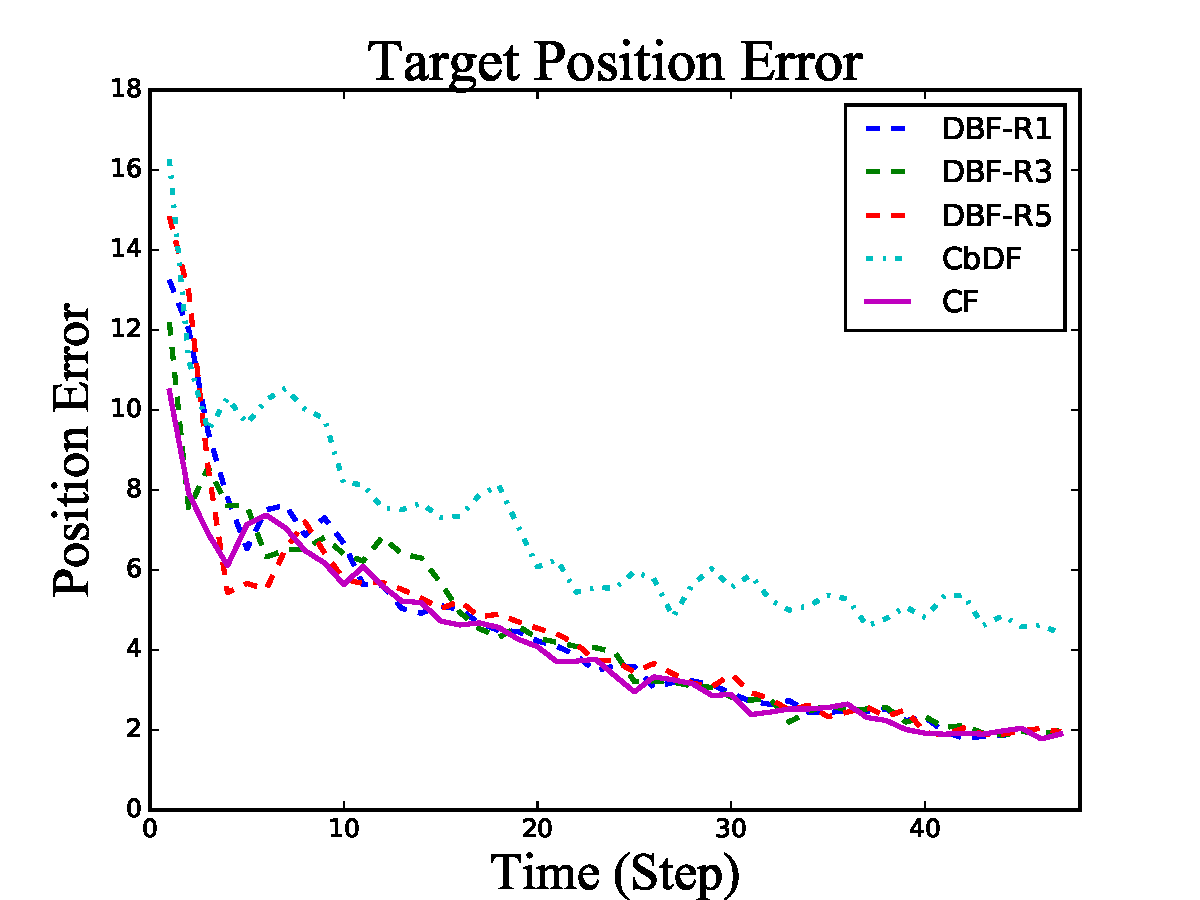
\includegraphics[width=\textwidth]{figures/brg_sta_sen_sta_tar_pos_err}
		\caption{Position Error}\label{fig:sta_sen_sta_tar_pos_err}
	\end{subfigure}
	\begin{subfigure}{0.23\textwidth}%[b]
		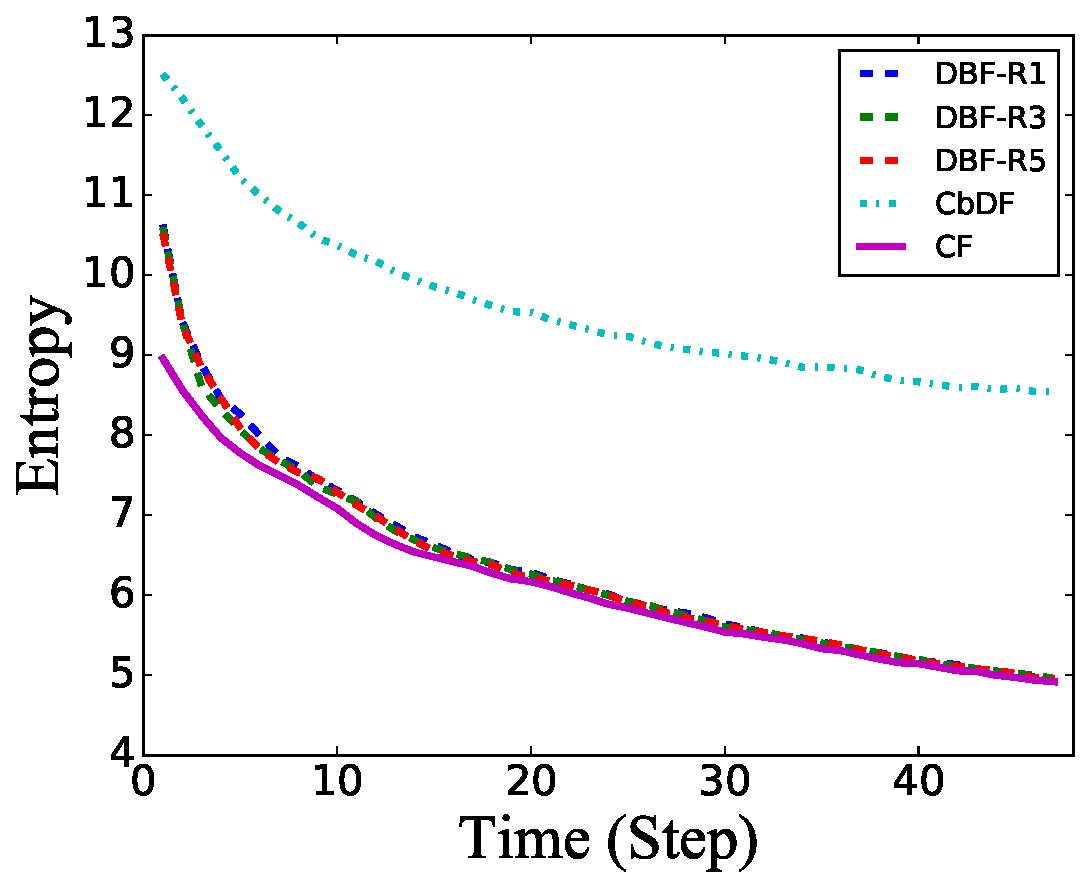
\includegraphics[width=\textwidth]		{figures/brg_sta_sen_sta_tar_entropy}%{figures/test2}
		\caption{Entropy of Individual PDF}\label{fig:sta_sen_sta_tar_entropy}
	\end{subfigure}
	\caption{(a)-(d) The $1^\text{st}$ UGV's individual PDF at different times. 
		%		The red star denotes the UGV whose individual PDF is shown. 
		The cross stands for the target. Note that the value of the color bar varies among different figures. (e) Average position estimation error of the $1^\text{st}$, $3^\text{rd}$ and $5^\text{th}$ UGV's LIFO-DBF, the CbDF and the CF. (f) Average entropy of individual PDFs.}
	\label{fig:sta_sen_sta_tar}
	%	\vspace{-1.2em}
\end{figure}

\begin{figure}%[h]
	\centering
	\begin{subfigure}{0.23\textwidth}%[b]
		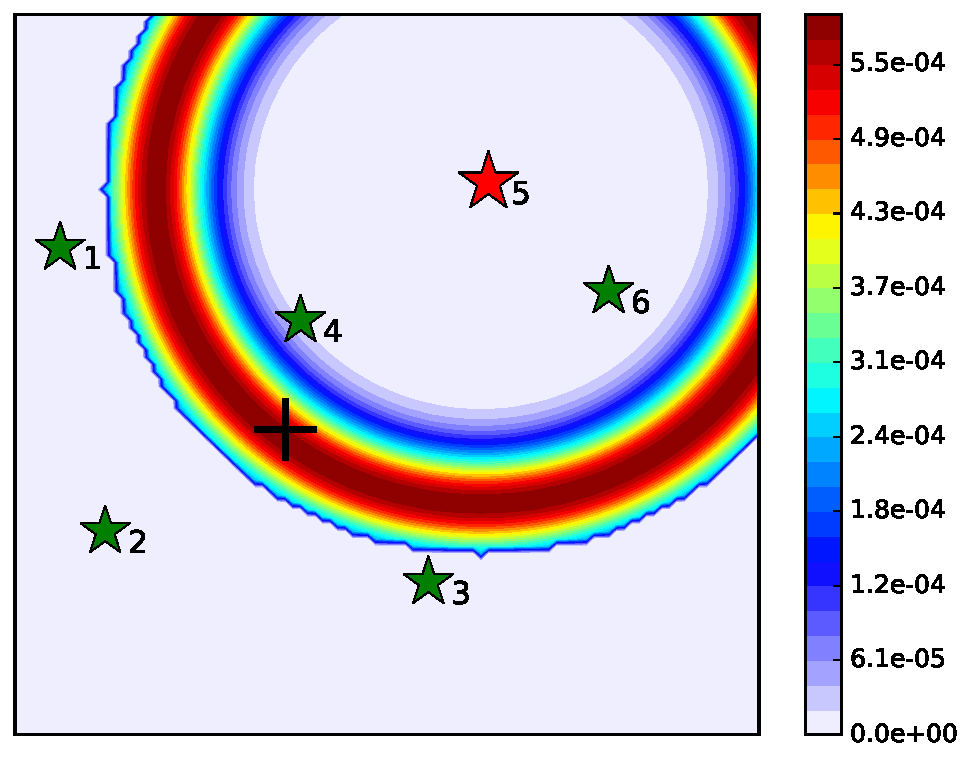
\includegraphics[width=\textwidth]{figures/hetero_sta_sen_sta_tar_rbt5_step1}
		\caption{Step 1}\label{fig:htr_sta_sen_sta_tar_sing1}
	\end{subfigure}
	\begin{subfigure}{0.23\textwidth}%[b]
		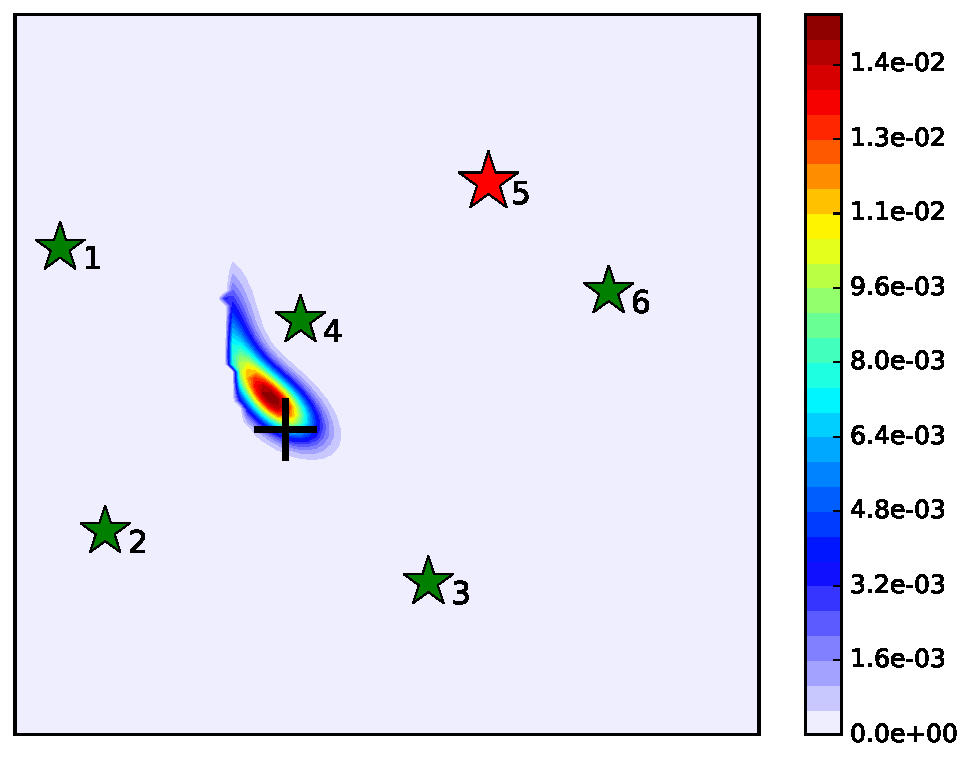
\includegraphics[width=\textwidth]{figures/hetero_sta_sen_sta_tar_rbt5_step3}
		\caption{Step 3}\label{fig:htr_sta_sen_sta_tar_sing2}
	\end{subfigure}
	\begin{subfigure}{0.23\textwidth}%[b]
		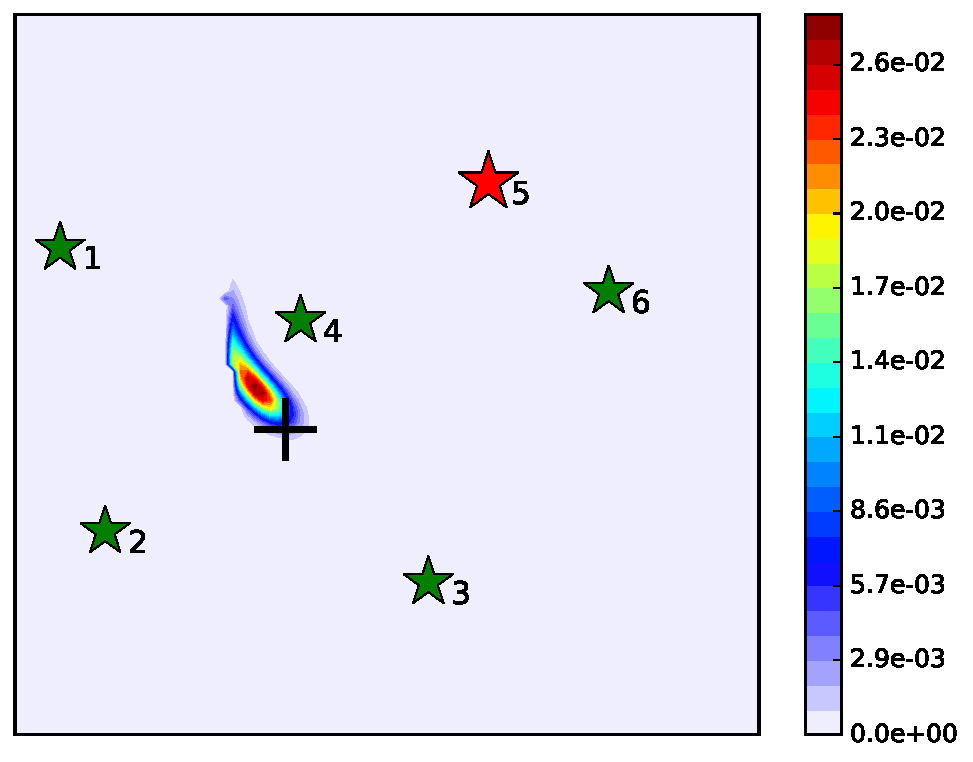
\includegraphics[width=\textwidth]{figures/hetero_sta_sen_sta_tar_rbt5_step5}
		\caption{Step 5}\label{fig:htr_sta_sen_sta_tar_sing3}
	\end{subfigure}
	\begin{subfigure}{0.23\textwidth}%[b]
		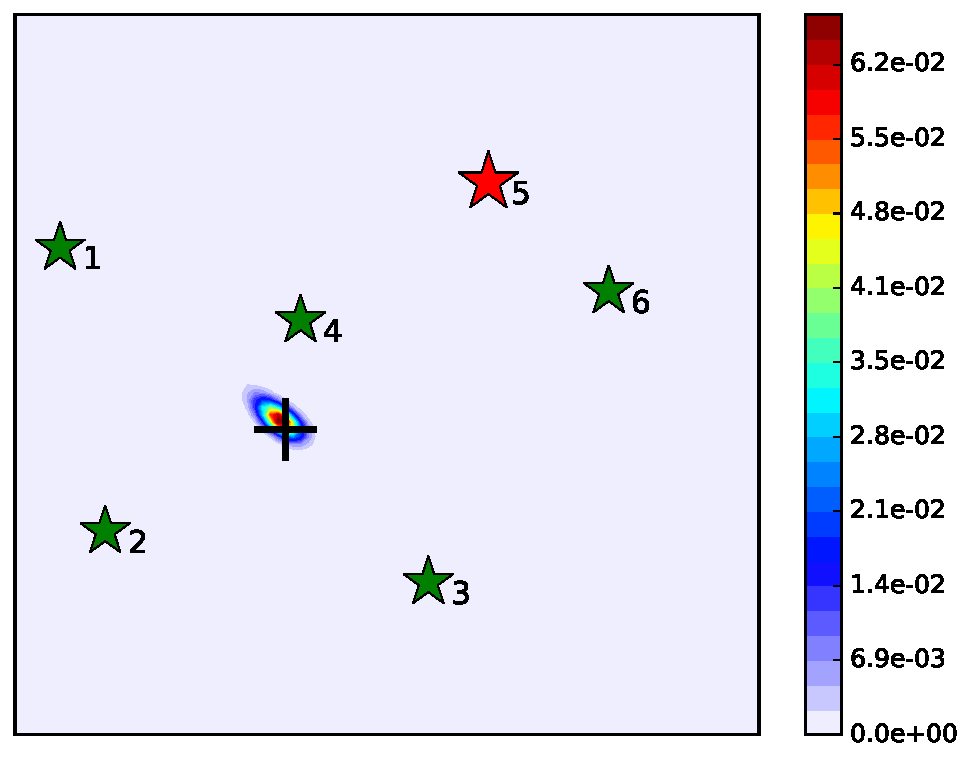
\includegraphics[width=\textwidth]{figures/hetero_sta_sen_sta_tar_rbt5_step10}
		\caption{Step 10}\label{fig:htr_sta_sen_sta_tar_sing4}
	\end{subfigure}
	\begin{subfigure}{0.23\textwidth}%[b]
		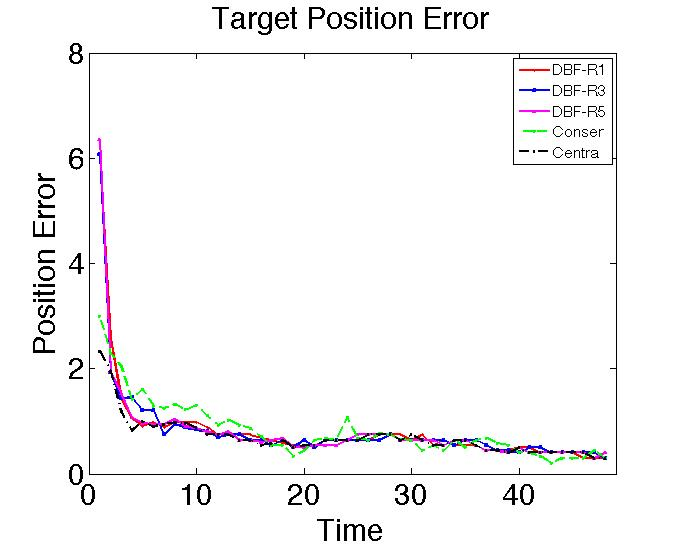
\includegraphics[width=\textwidth]{figures/hetero_sta_sen_sta_tar_pos_err}
		\caption{Position Error}\label{fig:htr_sta_sen_sta_tar_pos_err}
	\end{subfigure}
	\begin{subfigure}{0.23\textwidth}%[b]
		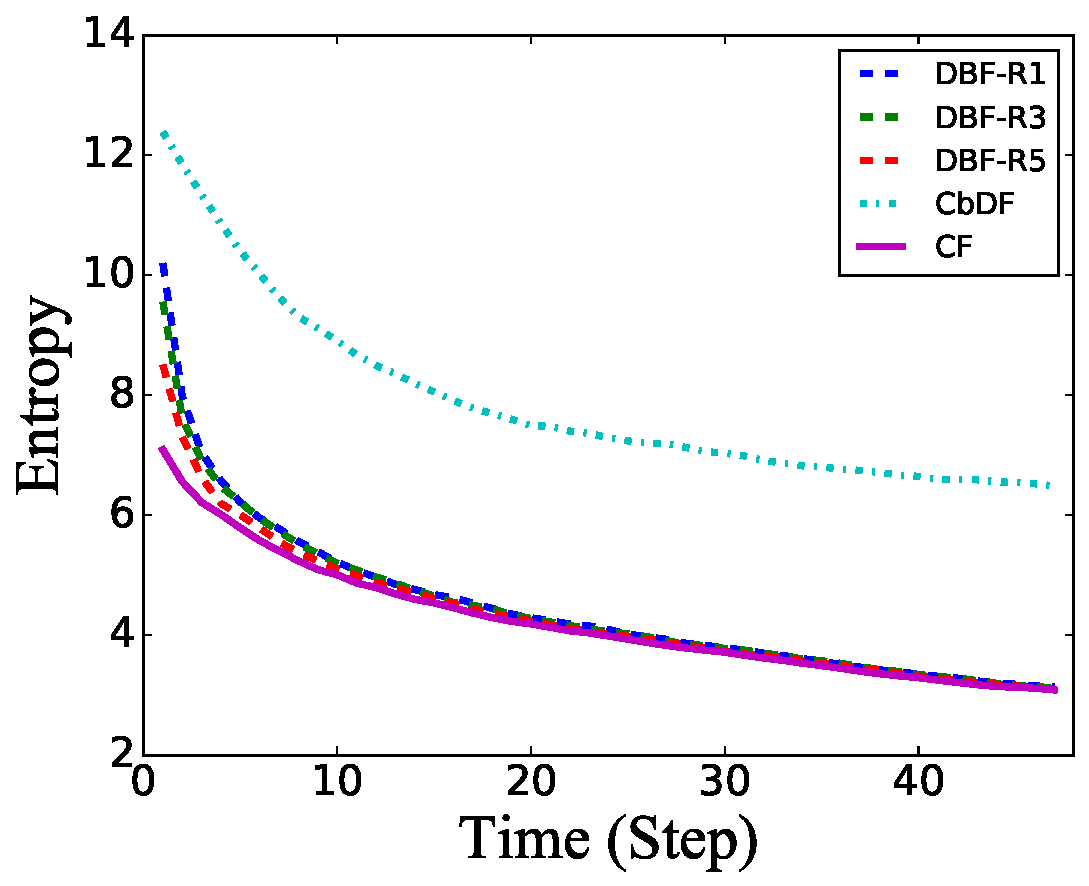
\includegraphics[width=\textwidth]{figures/hetero_sta_sen_sta_tar_entropy}
		\caption{Entropy of Individual PDF}\label{fig:htr_sta_sen_sta_tar_entropy}
	\end{subfigure}
	\caption{(a)-(d) The $5^\text{th}$ UGV's individual PDF at different times. (e) Average position estimation error. (f) Average entropy of individual PDFs.}
	\label{fig:htr_sta_sen_sta_tar}
	%	\vspace{-1.2em}
\end{figure}

\begin{figure}%[thpb]
	\centering
	\begin{subfigure}[b]{0.23\textwidth}
		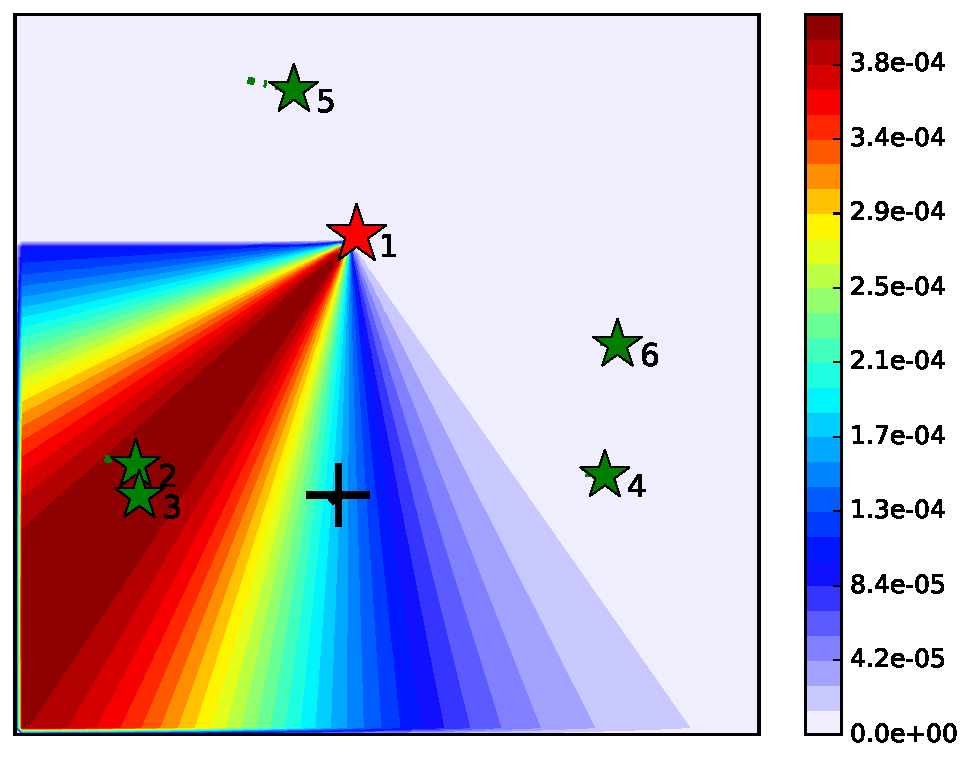
\includegraphics[width=\textwidth]{figures/brg_mov_sen_mov_tar_rbt1_step1}
		\caption{Step 1}\label{fig:mov_sen_mov_tar_sing1}
	\end{subfigure}
	\begin{subfigure}[b]{0.23\textwidth}
		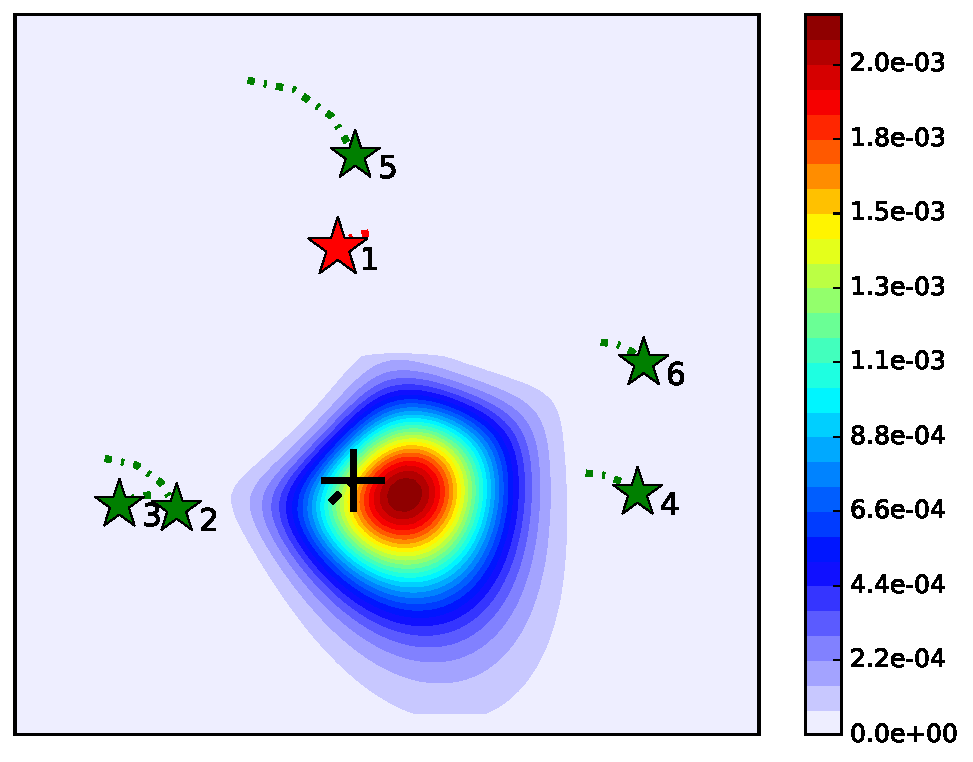
\includegraphics[width=\textwidth]{figures/brg_mov_sen_mov_tar_rbt1_step3}
		\caption{Step 3}\label{fig:mov_sen_mov_tar_sing2}
	\end{subfigure}	
	\begin{subfigure}[b]{0.23\textwidth}
		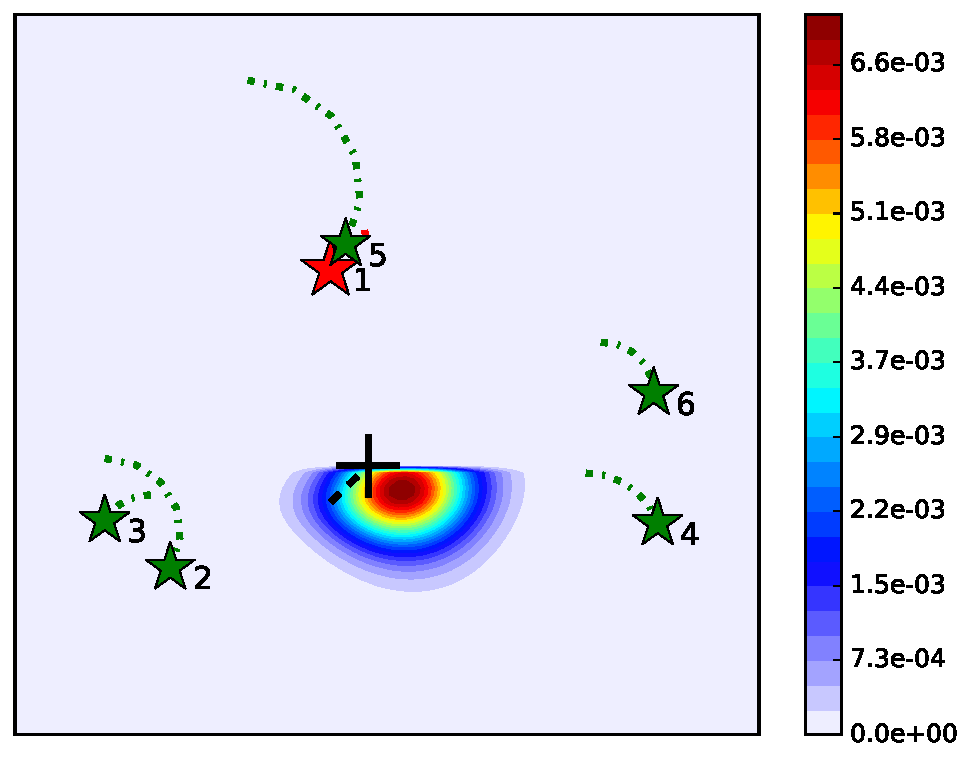
\includegraphics[width=\textwidth]{figures/brg_mov_sen_mov_tar_rbt1_step5}
		\caption{Step 5}\label{fig:mov_sen_mov_tar_sing3}
	\end{subfigure}	
	\begin{subfigure}[b]{0.23\textwidth}
		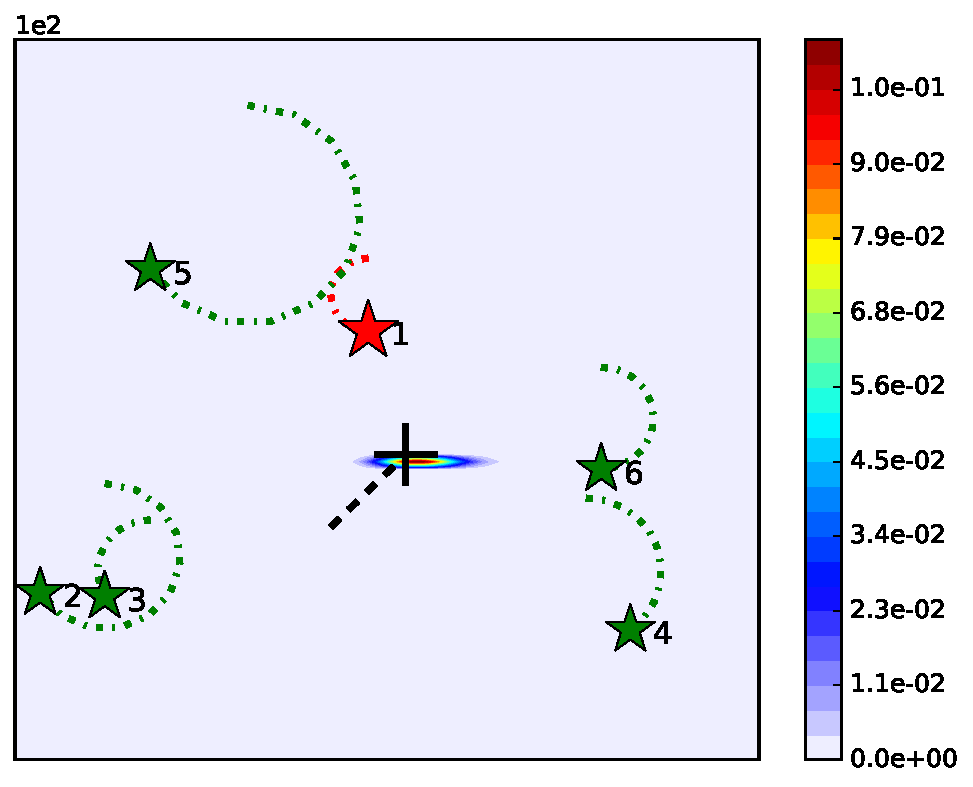
\includegraphics[width=\textwidth]{figures/brg_mov_sen_mov_tar_rbt1_step10}
		\caption{Step 10}\label{fig:mov_sen_mov_tar_sing4}
	\end{subfigure}
	\begin{subfigure}[b]{0.23\textwidth}
		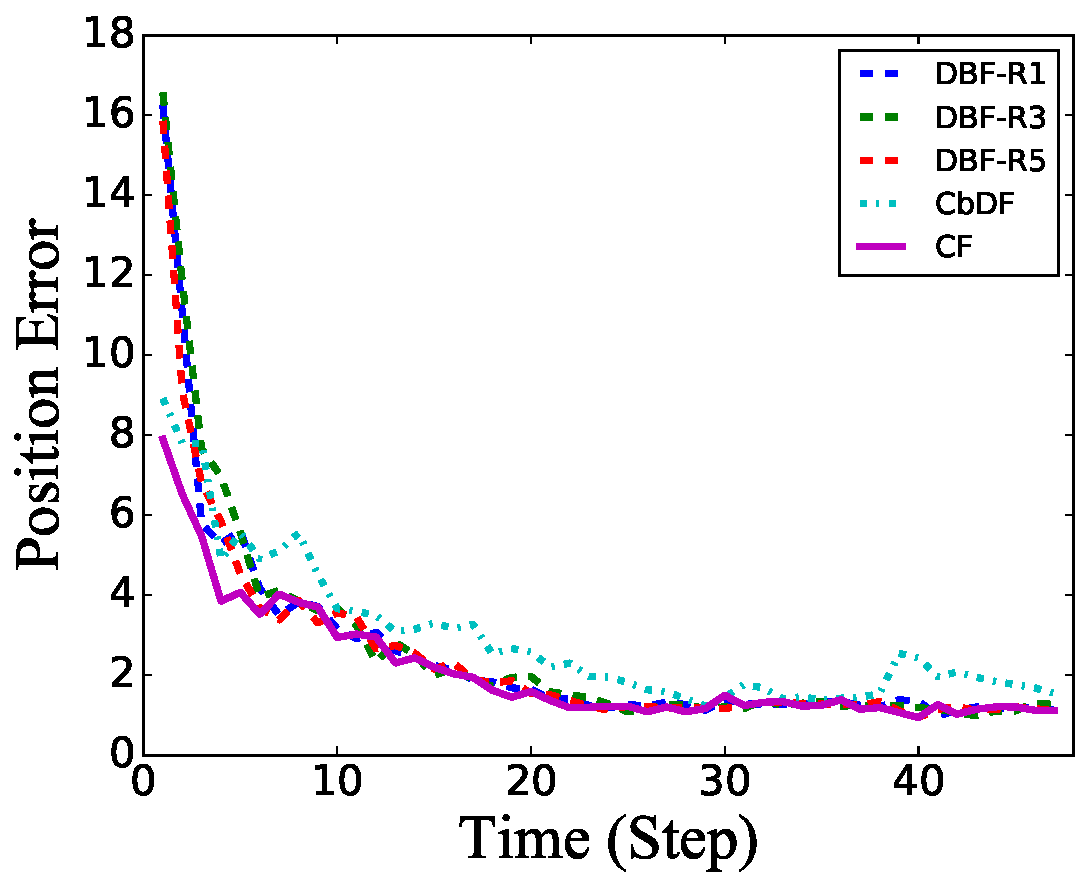
\includegraphics[width=\textwidth]{figures/brg_mov_sen_mov_tar_pos_err.pdf}
		\caption{Position Error}\label{fig:mov_sen_mov_tar_pos_err}
	\end{subfigure}
	\begin{subfigure}[b]{0.23\textwidth}
		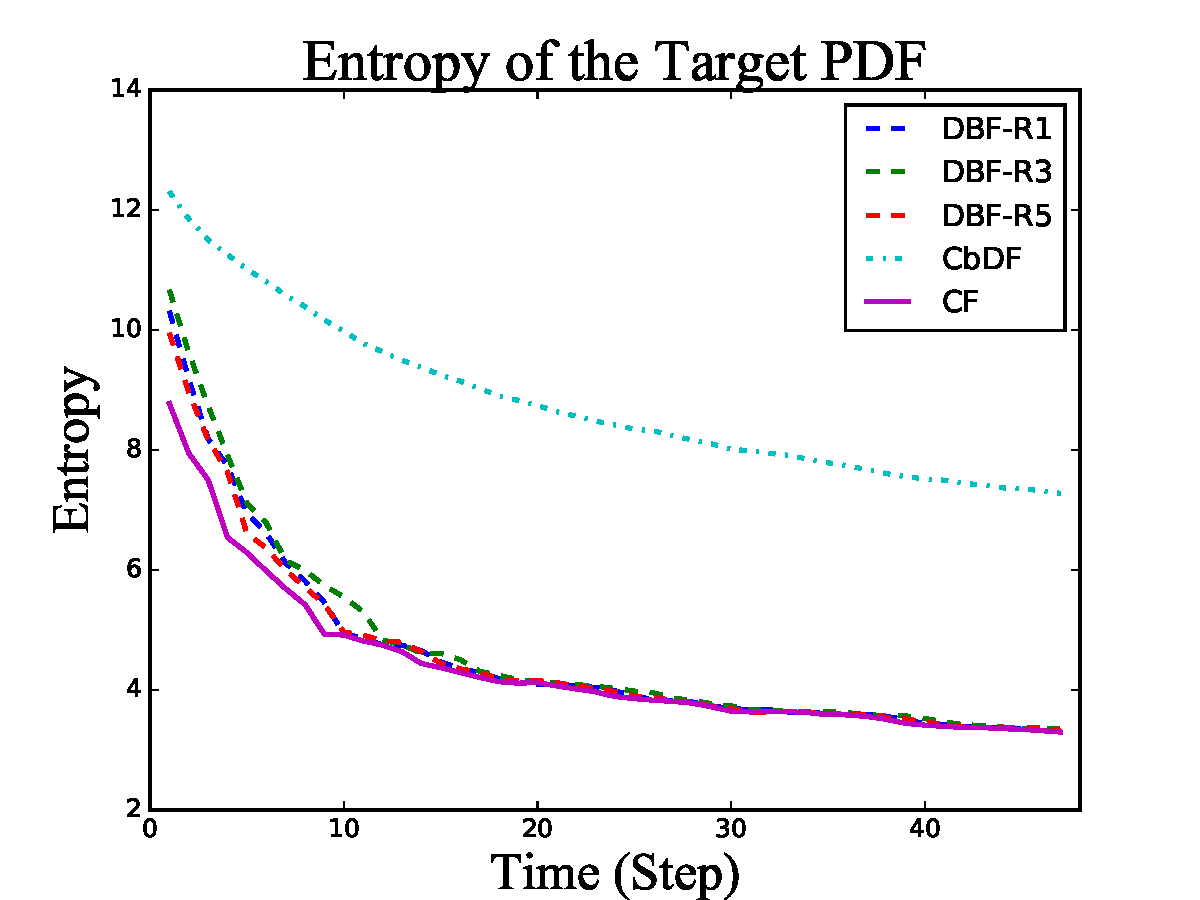
\includegraphics[width=\textwidth]{figures/brg_mov_sen_mov_tar_entropy.pdf}
		\caption{Entropy of Individual PDF}\label{fig:mov_sen_mov_tar_entropy}
	\end{subfigure}
	%	\begin{subfigure}[b]{0.4\textwidth}
	%		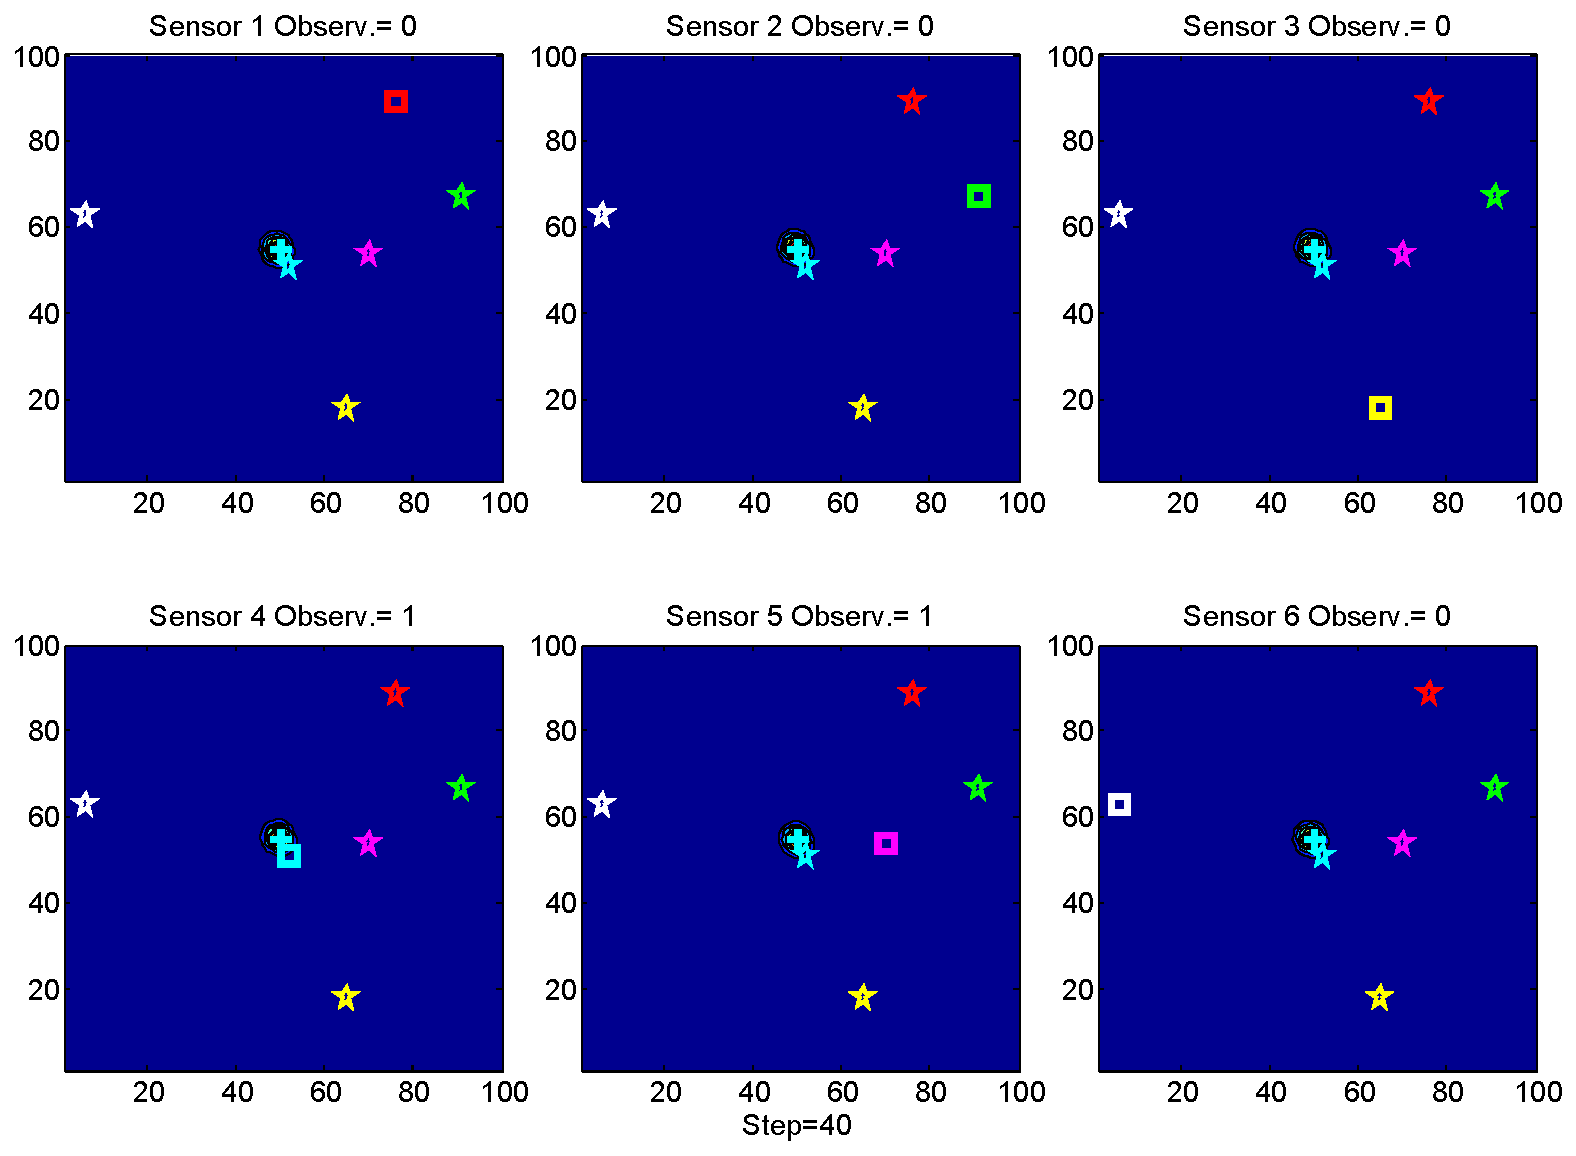
\includegraphics[width=\textwidth]{figures/mov_sen_mov_tar_40}
	%		\caption{Step 40}\label{fig:mov_sen_mov_tar_all}
	%	\end{subfigure}
	\caption{(a)-(d) The $1^\text{st}$ UGV's individual PDFs at different times. The green dashed lines represent robots' trajectories. (e) Average position estimation error. (f) Average entropy of individual PDFs.}
	\label{fig:mov_sen_mov_tar}
	%	\vspace{-1.1em}
\end{figure}

\begin{figure}%[thpb]
	\centering
	\begin{subfigure}[b]{0.23\textwidth}
		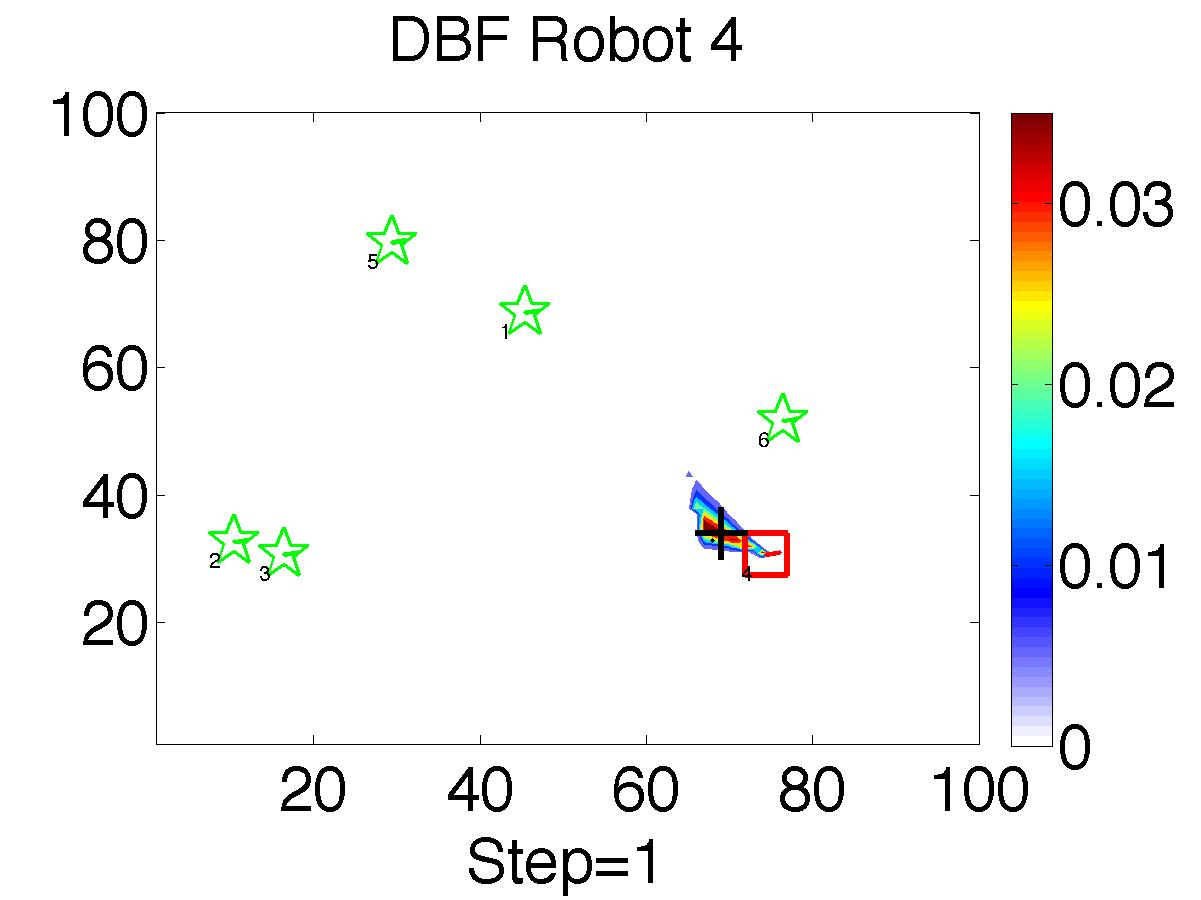
\includegraphics[width=\textwidth]{figures/hetero_mov_sen_mov_tar_rbt4_step1}
		\caption{Step 1}\label{fig:htr_mov_sen_mov_tar_sing1}
	\end{subfigure}
	\begin{subfigure}[b]{0.23\textwidth}
		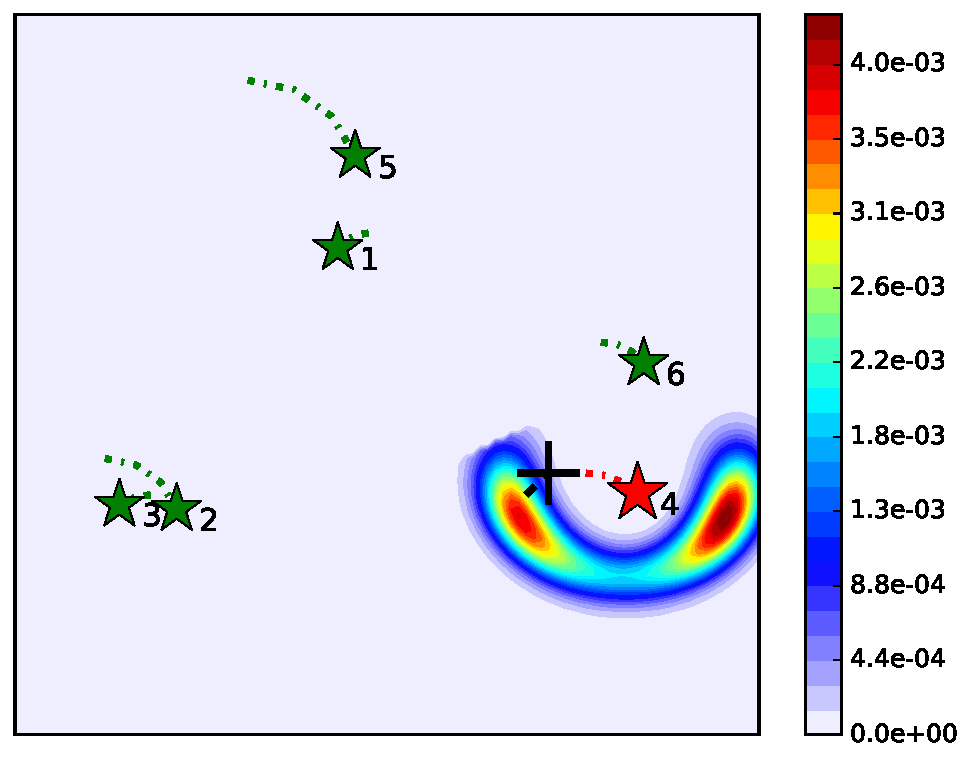
\includegraphics[width=\textwidth]{figures/hetero_mov_sen_mov_tar_rbt4_step3}
		\caption{Step 3}\label{fig:htr_mov_sen_mov_tar_sing2}
	\end{subfigure}
	\begin{subfigure}[b]{0.23\textwidth}
		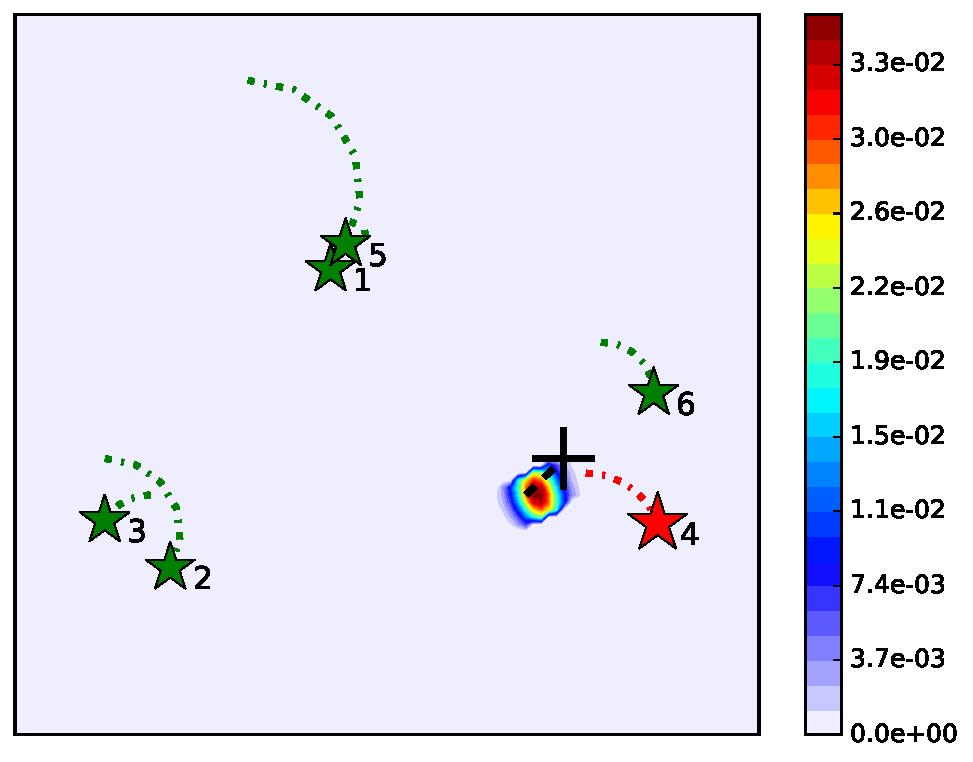
\includegraphics[width=\textwidth]{figures/hetero_mov_sen_mov_tar_rbt4_step5}
		\caption{Step 5}\label{fig:htr_mov_sen_mov_tar_sing3}
	\end{subfigure}
	\begin{subfigure}[b]{0.23\textwidth}
		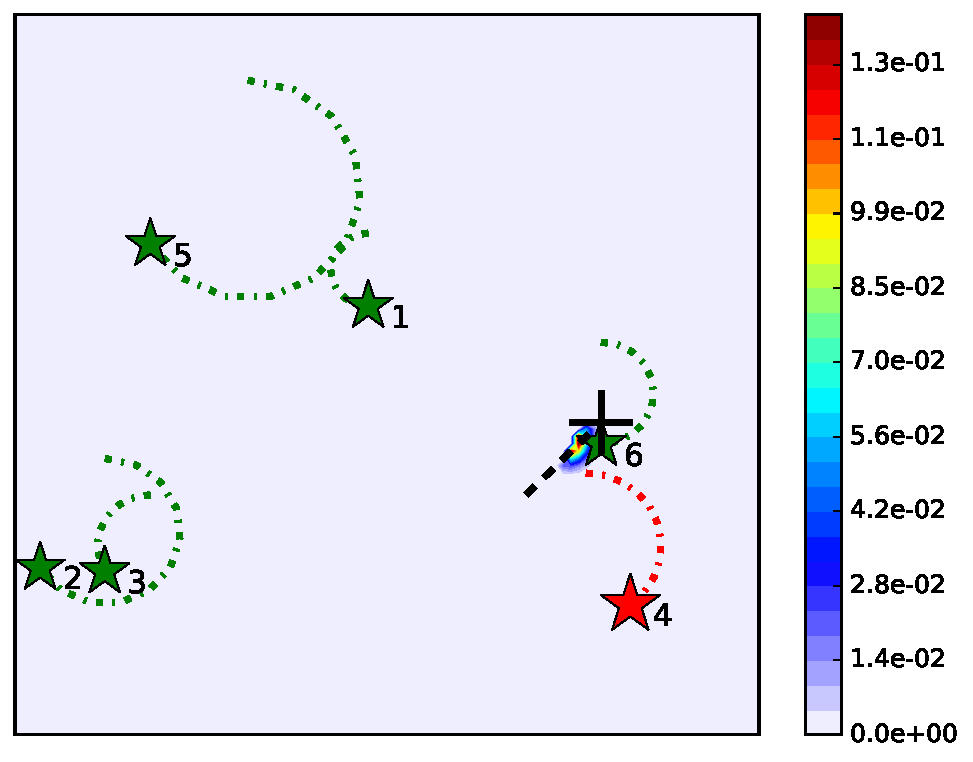
\includegraphics[width=\textwidth]{figures/hetero_mov_sen_mov_tar_rbt4_step10}
		\caption{Step 10}\label{fig:htr_mov_sen_mov_tar_sing4}
	\end{subfigure}
	\begin{subfigure}[b]{0.23\textwidth}
		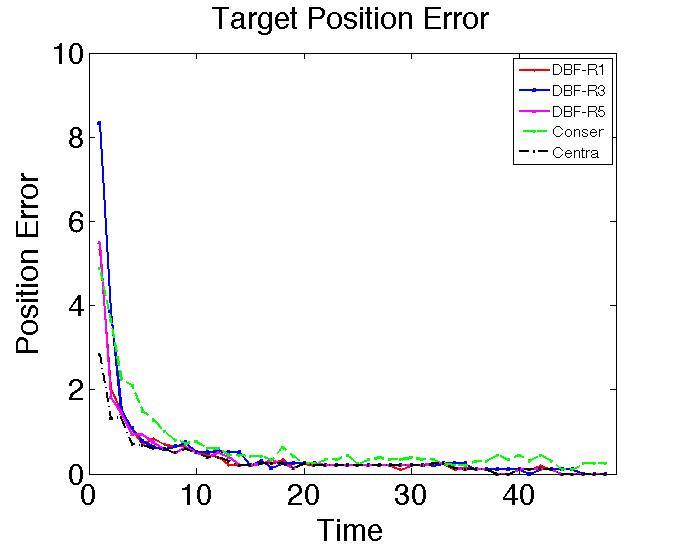
\includegraphics[width=\textwidth]{figures/hetero_mov_sen_mov_tar_pos_err}
		\caption{Position Error}\label{fig:htr_mov_sen_mov_tar_pos_err}
	\end{subfigure}
	\begin{subfigure}[b]{0.23\textwidth}
		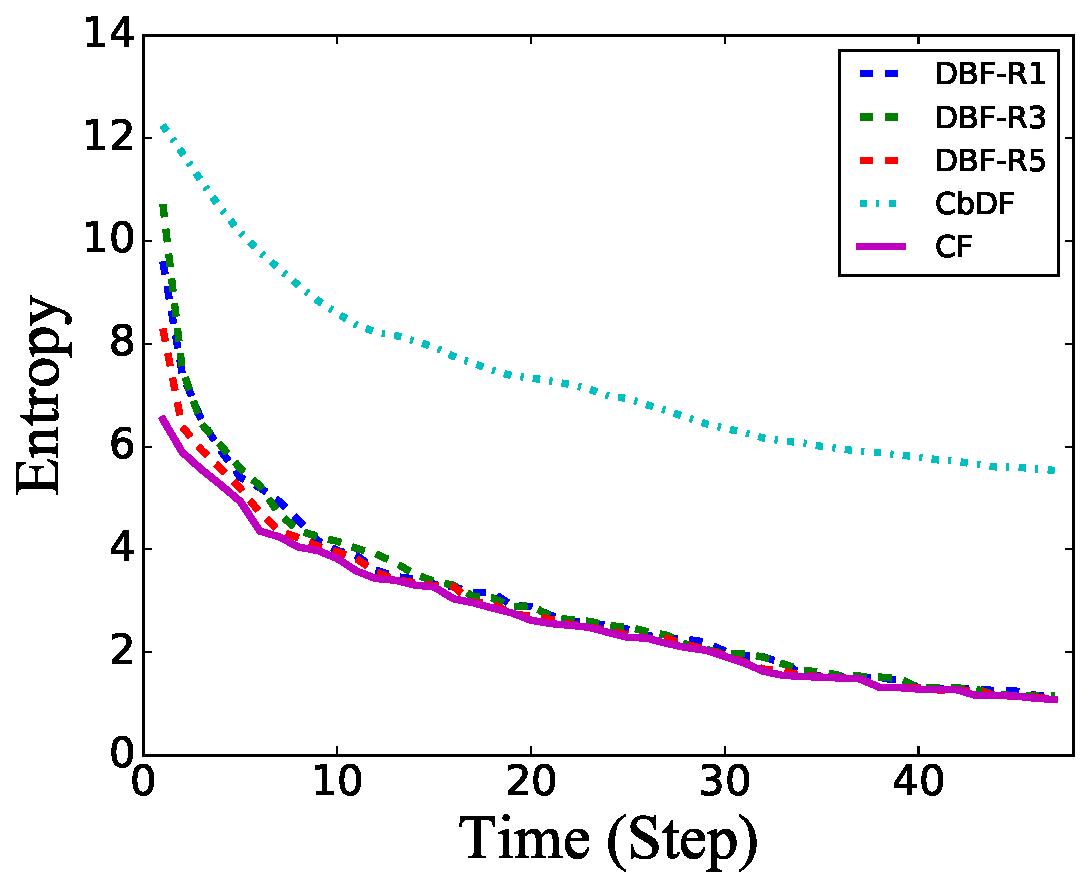
\includegraphics[width=\textwidth]{figures/hetero_mov_sen_mov_tar_entropy}
		\caption{Entropy of Individual PDF}\label{fig:htr_mov_sen_mov_tar_entropy}
	\end{subfigure}
	\caption{(a)-(d) The $4^\text{th}$ UGV's individual PDF at different times. (e) Average position estimation error. (f) Average entropy of individual PDFs.}
	%\label{fig:sta_sen_sta_tar}
	%	\vspace{-1.2em}
\end{figure}

\addtolength{\textheight}{0cm}   % This command serves to balance the column lengths
                                  % on the last page of the document manually. It shortens
                                  % the textheight of the last page by a suitable amount.
                                  % This command does not take effect until the next page
                                  % so it should come on the page before the last. Make
                                  % sure that you do not shorten the textheight too much.

%%%%%%%%%%%%%%%%%%%%%%%%%%%%%%%%%%%%%%%%%%%%%%%%%%%%%%%%%%%%%%%%%%%%%%%%%%%%%%%%
\bibliographystyle{IEEEtran}
%\bibliographystyle{bibtex}
\bibliography{references}

\end{document}
